\section{Issuing Queries on an Arrangement\label{arr_sec:queries}}
% ==============================================================================
One of the most important query types defined on arrangements is
the \emph{point-location} query: Given a point, find the arrangement
cell that contains it. Typically, the result of a point-location
query is one of the arrangement faces, but in degenerate situations
the query point can be located on an edge or it may coincide with a
vertex.

Point-location queries are common in many applications, and also
play an important role in the incremental construction of arrangements
(and more specifically in the free insertion-functions described in
Section~\ref{arr_sec:gl_funcs}). Therefore, it is crucial to have the
ability to answer such queries effectively.

\subsection{Point-Location Queries\label{arr_ssec:pl}}
% ------------------------------------------------------------------------------
The \ccc{Arrangement_2} class template does not support point-location
queries directly, as the arrangement representation is decoupled from
the geometric algorithms that operate on it. The \emph{2D Arrangements}
package includes a set of classe templates that are capable of
answering such queries; all are models of the concept
\ccc{ArrangementPointLocation_2}. Each model employs a different
algorithm or \emph{strategy} for answering queries. A model of this
concept must define the \ccc{locate()} member function, which accepts
an input query-point and returns an object that represents the
arrangement cell that contains this point. This object is is type
\ccc{Arr_point_location_result<Arrangement_2>::Type}---a discriminated
union container of the bounded types \ccc{Vertex_const_handle},
\ccc{Halfedge_const_handle}, or \ccc{Face_const_handle}. Depending on
whether the query point is located inside a face, on an edge, or on a
vertex, the appropriate handle can be obtained With \emph{value retrieval}
by \ccc{boost::get} as demonstrated in the example below.

Note that the handles returned by the \ccc{locate()} functionss are
non-mutable (\ccc{const}). If necessary, such handles may
be cast to mutable handles using the \ccc{non_const_handle()} methods
\ccc{Arrangement_2::non_const_handle()} provided by the
\ccc{Arrangement_2} class.

An object \ccc{pl} of any point-location class must be attached to an
\ccc{Arrangement_2} object \ccc{arr} before it is used to answer
point-location queries on \ccc{arr}. This attachment can be performed
when \ccc{pl} is constructed or at a later time using the
\ccc{pl.init(arr)} call.

The function template listed below accepts a point-location object,
the type of which is a model of the \ccc{ArrangementPointLocation_2}
concept, and a query point. The function template issues a
point-location query for the given point, and prints out the result.
It is defined in the header file \ccc{point_location_utils.h}.

\label{lst:pl}
\begin{alltt}
template <typename PointLocation>
void locate_point(const PointLocation& pl,
                  const typename PointLocation::Arrangement_2::Point_2& q)
\{
  typedef PointLocation                                 Point_location;
  typedef typename Point_location::Arrangement_2        Arrangement_2;
  typename CGAL::Arr_point_location_result<Arrangement_2>::Type obj =
    pl.locate(q);

  // Print the result.
  print_point_location<Arrangement_2>(q, obj);
\}
\end{alltt}

The function template \ccc{locate_point()} calls an instance of the
function template \ccc{print_point_location()}, which inserts the
result of the query into the standard output-stream. It is listed
below, and defined in the header file \ccc{point_location_utils.h}.
Observe how the function \ccc{boost::get()} is used to cast the
resulting object into a handle to an arrangement feature. The
point-location object \ccc{pl} is assumed to be already attached
to an arrangement.

\begin{alltt}
template <typename Arrangement_>
void
print_point_location
(const typename PointLocation::Arrangement_2::Point_2& q
 typename CGAL::Arr_point_location_result<Arrangement_>::Type obj)
\{
  typedef Arrangement_                                  Arrangement_2;
  
  typedef typename Arrangement_2::Vertex_const_handle   Vertex_const_handle;
  typedef typename Arrangement_2::Halfedge_const_handle Halfedge_const_handle;
  typedef typename Arrangement_2::Face_const_handle     Face_const_handle;

  const Vertex_const_handle*   v;
  const Halfedge_const_handle* e;
  const Face_const_handle*     f;

  std::cout << "The point (" << q << ") is located ";
  if (f = boost::get<Face_const_handle>(&obj))         // located inside a face
    std::cout << "inside "
              << (((*f)->is_unbounded()) ? "the unbounded" : "a bounded")
              << " face." << std::endl;
  else if (e = boost::get<Halfedge_const_handle>(&obj)) // located on an edge
    std::cout << "on an edge: " << (*e)->curve() << std::endl;
  else if (v = boost::get<Vertex_const_handle>(&obj))   // located on a vertex
    std::cout << "on " << (((*v)->is_isolated()) ? "an isolated" : "a")
              << " vertex: " << (*v)->point() << std::endl;
  else CGAL_error_msg("Invalid object.");
\}
\end{alltt}

\subsubsection{Choosing a Point-Location Strategy\label{arr_sssec:pl_strat}}
% ------------------------------------------------------------------------------
Each of the various point-location class templates employs a different
algorithm or \emph{strategy}\footnote{The term \emph{strategy}
is borrowed from the design-pattern
taxonomy~\cite[Chapter~5]{ghjv-dp-95}.} for answering queries:
\begin{itemize}
\item \ccc{Arr_naive_point_location<Arrangement>} employes the
  \emph{naive} strategy. It locates the query point naively,
  exhaustively scanning all arrangement cells.
  %
\item \ccc{Arr_walk_along_a_line_point_location<Arrangement>} employs
  the \emph{walk-along-a-line} (or \emph{walk} for short) strategy.
  It simulates a traversal, in reverse order, along an imaginary
  vertical ray emanating from the query point. It starts from the
  unbounded face of the arrangement and moves downward toward the
  query point until locating the arrangement cell containing it.
  %
\item \ccc{Arr_landmarks_point_location<Arrangement,Generator>}
  uses a set of ``landmark'' points the location of which in the
  arrangement is known. It employs the
  \emph{landmark} strategy. Given a query point, it uses a
  nearest-neighbor search-structure (a \kdtree{} is used by default)
  to find the nearest landmark and then traverses the straight-line
  segment connecting this landmark to the query point.

  There are various ways to select the landmark set in the
  arrangement. The selection is governed by the \ccc{Generator}
  template parameter. The default generator class, namely
  \ccc{Arr_landmarks_vertices_generator}, selects all the vertices of
  the attached arrangement as landmarks. Additional generators that
  select the set in other ways, such as by sampling random
  points or choosing points on a grid, are also available; see the
  Reference Manual for more details.

  The landmark strategy requires that the type of the attached
  arrangement be an instance of the \ccc{Arrangement_2<Traits,Dcel>}
  class template, where the \ccc{Traits} parameter is substituted with
  a geometry-traits class that models the
  \ccc{ArrangementLandmarkTraits_2} concept, which refines the basic
  \ccc{ArrangementBasicTraits_2} concept; see
  Section~\ref{arr_sssec:tr_lanmarks_concept} for details. Most traits
  classes included in the \emph{2D Arrangement} package are models of
  this refined concept.
  %
\item \ccc{Arr_trapezoid_ric_point_location<Arrangement>} implements
  Mulmuley's point-location algorithm~\cite{m-fppa-90}; see
  also~\cite[Chapter~6]{bkos-cgaa-00}). The arrangement faces are
  decomposed into simpler cells each of constant complexity, known as
  \emph{pseudo-trapezoids}, and a search structure (a directed acyclic
  graph) is constructed on top of these cells, facilitating the search
  of the pseudo trapezoid (hence the arrangement cell) containing a
  query point in expected logarithmic time. The trapezoidal map and
  the search structure are built by a algorithm (RIC).
\end{itemize}

The first two strategies do not require any extra data. The class
templates that implement them store a pointer to an arrangement object
and operate directly on it. Attaching such point-location objects to
an existing arrangement has virtually no running-time cost at all, but
the query time is linear in the size of the arrangement (the
performance of the walk strategy is much better in practice, but
its worst-case performance is linear). Using these strategies is
therefore recommended only when a relatively small number of
point-location queries are issued by the application, or when the
arrangement is constantly changing (That is, changes in the arrangement
structure are more frequent than point-location queries).

On the other hand, the landmarks and the trapezoid RIC strategies
require auxiliary data structures on top of the arrangement, which
they need to construct once they are attached to an arrangement
object and need to keep up-to-date as this arrangement changes.
The data structures needed by both strategies can be constructed
in $O(N \log N)$ time, where $N$ is the overall number of edges in
the arrangement, but the constant hidden in the $O()$ notation for the
trapezoidal map RIC strategy is much larger. Thus, construction needed
by the landmark algorithm is in practice significantly faster than the
construction needed by the trapezoidal map RIC strategy. In addition,
although both resulting data structures are asymptotically linear in
size, using a \kdtree{} as the nearest-neighbor search-structure that
the landmark algorithm stores significantly reduces memory consumption.
The trapezoidal map RIC algorithm has expected logarithmic query time,
while the query time for the landmark strategy may be as large as
linear. In practice however, the query times of both strategies are
competitive. For a detailed experimental comparison
see~\cite{cgal:hh-eplca-05}

Updating the auxiliary data structures of the trapezoidal map RIC
algorithm is done very efficiently. On the other hand, updating the
nearest-neighbor search-structure of the landmark algorithm may consume
more time when the arrangement changes frequently, especially when
a \kdtree{} is used, as it must be rebuilt each time the arrangement
changes. It is therefore recommended that the
\ccc{Arr_landmarks_point_location} class template be used when the
application frequently issues point-location queries on an arrangement
that only seldom changes. If the arrangement is more dynamic and is
frequently going through changes, the \ccc{Arr_trapezoid_ric_point_location}
class template should be the selected point-location strategy.

\subsubsection{An Example\label{arr_sssec:pl_ex}}
% ------------------------------------------------------------------------------
\begin{figure}[t]
\begin{ccTexOnly}
  \begin{center}
  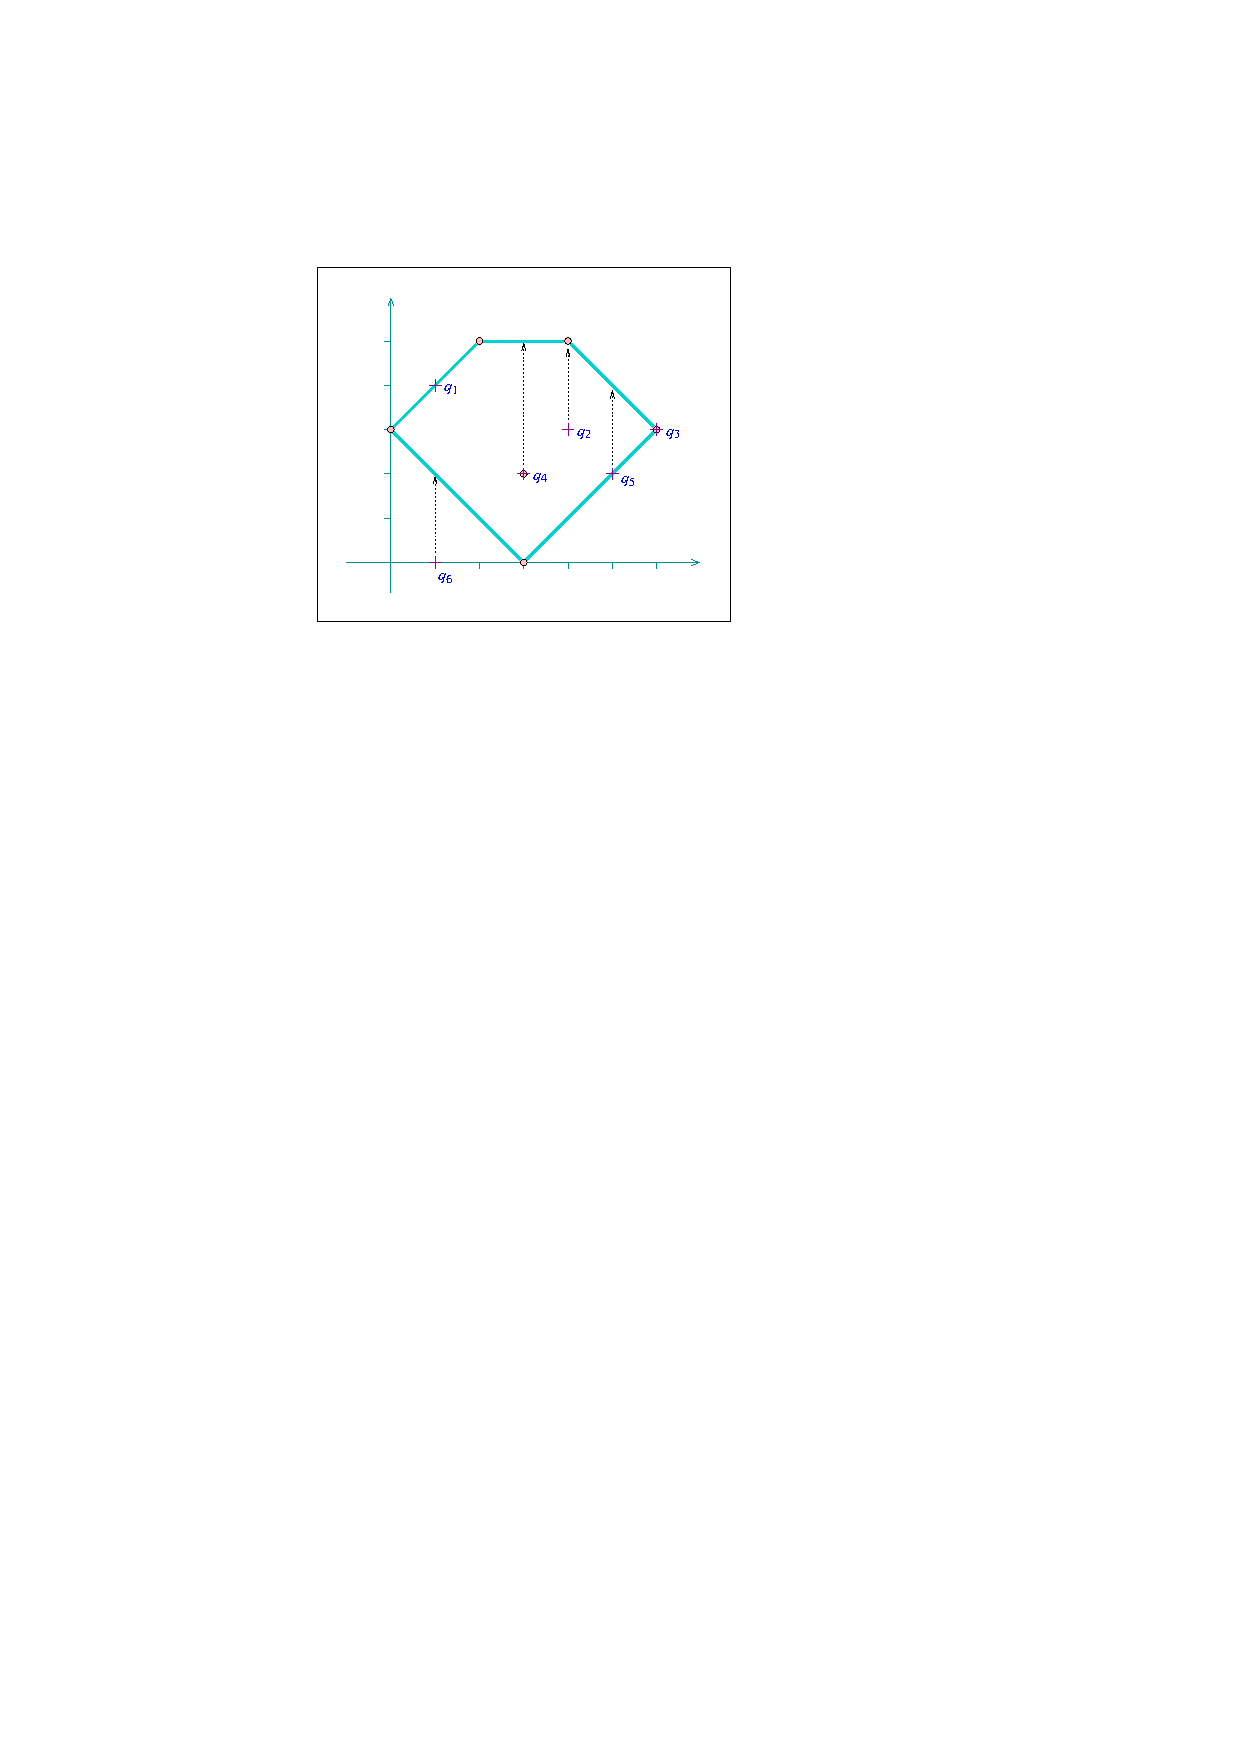
\includegraphics{Arrangement_on_surface_2/fig/ex_5}
  \end{center}
\end{ccTexOnly}
\begin{ccHtmlOnly}
  <p><center>
  <img src="./fig/ex_5.gif" border=0 alt="Example 5">
  </center>
\end{ccHtmlOnly}
\caption{The arrangement of line segments, as constructed in
\ccc{point_location.cpp}, \ccc{vertical_ray_shooting.cpp}, and
\ccc{batched_point_location.cpp}. The
arrangement vertices are drawn as small discs, while the query
points $q_1, \ldots, q_6$ are marked with crosses.\label{arr_fig:ex_5}}
\end{figure}

The program listed below constructs a simple arrangement of five line
segments that form a pentagonal face, with a single isolated
vertex in its interior, as depicted in Figure~\ref{arr_fig:ex_5}.
Notice that we use the same arrangement structure in the next
three example programs. The arrangement construction is performed by
the function \ccc{construct_segment_arr()} defined in the heade file
\ccc{point_location_utils.h}. (Its listing is omitted here.) The
program employs the naive and the landmark strategies to issue
several point-location queries on this arrangement.

\ccIncludeExampleCode{Arrangement_on_surface_2/point_location.cpp}

Note that the program uses the \ccc{locate_point()} function template
to locate a point and nicely print the result of each query; see
Page~\pageref{lst:pl}.

\subsection{Vertical Ray Shooting\label{arr_ssec:ray_shoot}}
% ------------------------------------------------------------------------------
Another query frequently issued on arrangements is the vertical
ray-shooting query: Given a query point, which arrangement feature
do we encounter by a vertical ray shot upward (or downward) from this
point? In the general case the ray hits an edge, but it is possible
that it hits a vertex, or that the arrangement does not have any
vertex or edge lying directly above (or below) the query point.

All point-location classes listed in the previous section are also
models of the \ccc{ArrangementVerticalRayShoot_2} concept. That is,
they all have member functions called \ccc{ray_shoot_up(q)} and
\ccc{ray_shoot_down(q)} that accept a query point $q$. These functions
output an object of type type
\ccc{Arr_point_location_result<Arrangement_2>::Type}---a discriminated
union container of the bounded types \ccc{Vertex_const_handle},
\ccc{Halfedge_const_handle}, or \ccc{Face_const_handle}. The latter type
is used for the unbounded face of the arrangement, in case there is no
edge or vertex lying directly above (or below) $q$.

The function template \ccc{vertical_ray_shooting_query()} listed
below accepts a vertical ray-shooting object, the type of which
models the \ccc{ArrangementVerticalRayShoot_2} concept. It exports
the result of the upward vertical ray-shooting operation from a
given query point to the standard output-stream. The ray-shooting
object \ccc{vrs} is assumed to be already attached to an arrangement.
The function template is defined in the header file
\ccc{point_location_utils.h}.

\begin{alltt}
template <typename RayShoot>
void shoot_vertical_ray(const RayShoot& vrs,
                       const typename RayShoot::Arrangement_2::Point_2& q)
\{
  typedef RayShoot                                      Vertical_ray_shooting;

  // Perform the point-location query.
  typename Vertical_ray_shooting::result_type obj = vrs.ray_shoot_up(q);

  // Print the result.
  typedef typename Vertical_ray_shooting::Arrangement_2 Arrangement_2;
  typedef typename Arrangement_2::Vertex_const_handle   Vertex_const_handle;
  typedef typename Arrangement_2::Halfedge_const_handle Halfedge_const_handle;
  typedef typename Arrangement_2::Face_const_handle     Face_const_handle;

  const Vertex_const_handle*   v;
  const Halfedge_const_handle* e;
  const Face_const_handle*     f;
  
  std::cout << "Shooting up from (" << q << ") : ";
  if (v = boost::get<Vertex_const_handle>(&obj))            // we hit a vertex
    std::cout << "hit " << (((*v)->is_isolated()) ? "an isolated" : "a")
              << " vertex: " << (*v)->point() << std::endl;
  else if (e = boost::get<Halfedge_const_handle>(&obj))     // we hit an edge
    std::cout << "hit an edge: " << (*e)->curve() << std::endl;
  else if (f = boost::get<Face_const_handle>(&obj)) \{      // we hit nothing
    CGAL_assertion((*f)->is_unbounded());
    std::cout << "hit nothing." << std::endl; 
  \}
  else CGAL_error();
\}
\end{alltt}

The program below uses the function template listed above to
perform vertical ray-shooting queries on an arrangement. The
arrangement and the query points are exactly the same as in
\ccc{point_location.cpp}; see Figure~\ref{arr_fig:ex_5}.:

\ccIncludeExampleCode{Arrangement_on_surface_2/vertical_ray_shooting.cpp}

The number type we use in this example is \cgal's built-in
\ccc{MP_Float} type, which is a floating-point number with an
unbounded mantissa and a 32-bit exponent. It supports construction
from an integer or from a machine \ccc{float} or \ccc{double} and
performs additions, subtractions and multiplications in an exact
number.

\subsection{Batched Point-Location\label{arr_ssec:batched_pl}}
% ------------------------------------------------------------------------------
Suppose that at a given moment our application has to issue a
relatively large number $m$ of point-location queries on a
specific arrangement object. Naturally, It is possible to define
a point-location object and use it to issue separate queries on
the arrangement. However, as explained in Section~\ref{arr_ssec:pl},
choosing a simple point-location strategy (either the naive or
the walk strategy) means inefficient queries, while the more
sophisticated strategies need to construct auxiliary structures
that incur considerable overhead in running time.

Alternatively, the \emph{2D Arrangement} package includes a free
\ccc{locate()} function that accepts an arrangement and a range of
query points as its input and sweeps through the arrangement to
locate all query points in one pass. The function outputs the query
results as pairs, where each pair consists of a query point
and a discriminated union container, which represents the
cell containing the point; see Section~\ref{arr_ssec:pl}. The output
pairs are sorted in increasing $xy$-lexicographical order of the
query point.

The batched point-location operation is carried out by sweeping the
arrangement. Thus, it takes $O((m+N)\log{(m+N)})$  time, where $N$
is the number of edges in the arrangement. Issuing separate queries
exploiting a point-location strategy with logarithmic query time
per query, such as the trapezoidal map RIC strategy (see
Section~\ref{sssec:free:pl:strategy}), is asymptotically more
efficient. However, experiments show that when the number $m$ of
point-location queries is of the same order of magnitude as $N$,
the batched point-location operation is more efficient in practice. 
One of the reasons for the inferior performance of the alternative
(asymptotically faster) procedures is the necessity to construct
and maintain complex additional data structures.

The program below issues a batched point-location query, which
is essentially equivalent to the six separate queries performed in
\ccc{point_location.cpp};see Section~\ref{arr_ssec:pl}.

\ccIncludeExampleCode{Arrangement_on_surface_2/batched_point_location.cpp}
